\section{Atributo}
\label{sec:atributo}

Los atributos son los elementos utilizados en el standard UML para designar
propiedades que son inherentes a las clases, una vez instanciadas (las clases)
estos (los atributos) toman valor y ayudan al manejo de datos del objeto; El
lenguaje propuesto, permite el manejo de los atributos y algunas otras
cuestiones que están relacionadas con estos.

La definición de un atributo según notacion BNF es la siguiente:

\begin{lstlisting}[caption={BNF - Atributo}, basicstyle=\footnotesize\ttfamily]
  <atributo> ::= <visibilidad> <nombre> ":" <tipo>
\end{lstlisting}

Este elemento dentro del lenguaje se puede ver en un gráficamente en
un autómata finito de la siguiente manera:

\begin{figure}[H]
	\centering
	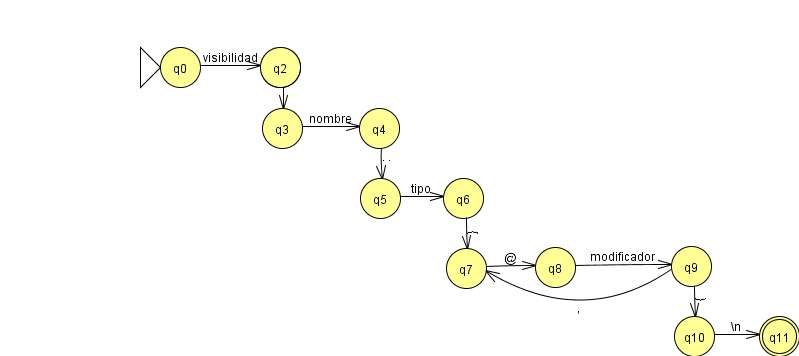
\includegraphics[width=.7\linewidth]{automatas_finitos/atributoDrt.png}
	\caption{Autómata finito - Atributo con restricciones de objeto}
	\label{fig:af_atr_modif}
\end{figure}

Teniendo en cuenta que el atributo tiene que estar definido dentro de otra
estructura del estándar UML, una clase.

A continuación un ejemplo, para expresar medianamente el funcionamiento del
lenguaje:\\

\begin{displayquote}
	\texttt{Consigna}: \textit{se desea tener una clase que permita el manejo de
	información de una persona, la información a manejar es el nombre, apellido
	y DNI}.
\end{displayquote}

Lo cual se puede representar mediante un diagrama de clase
de la siguiente manera:

\begin{figure}[H]
	\centering
	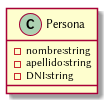
\includegraphics[width=.2\linewidth]{diagramas_clases/ej_diag_clase.png}
	\caption{Diagrama de Clase - representación de la consigna}
	\label{fig:ej_diag_clase.png}
\end{figure}

Teniendo esta información se puede armar un modelo en el lenguaje Director que
concuerde con estos requerimientos.

\textit{Dado a que por el momento unicamente se está tratando con los atributos
no se tendrá en cuenta la declaración de la clase \texttt{Persona} mencionada
en la consigna propuesta}.

\begin{lstlisting}[caption={Director - Modelado de atributos}, label=lst:atributo]
  ...
		private nombre:string
		private apellido:string
		private DNI:string
	...
\end{lstlisting}

Lo expuesto en el \texttt{Fragmento \ref{lst:atributo}}, demuestra
la capacidad del lenguaje de describir una serie de atributos con sus
respectivos metadatos (visibilidad y tipo), sin embargo, cabe destacar que
también se deja abierta la posibilidad de la futura implementación y
la compatibilización con funcionalidades relacionadas al Lenguaje de
Restricción de Objetos, puesto a que la adición de éstas
características automatizaria aún más el proceso de
desarrollo y permitiría el pase de modelo-a-código de manera mas sencilla.

Las características que se implementan compatibles funcionalidades brindadas
por OCL son las de modificadores para los atributos, estos modificadores ya
se mencionaron en la \texttt{Sección \ref{sec:palabrasreservadas}}.

Como ejemplo, se podrían aplicar algunas de estas cuestiones a lo implementado
en \texttt{Fragmento \ref{lst:atributo}} resultando lo siguiente:

\begin{lstlisting}[caption={Director - Modelao de atributos (con OCL)},
label=lst:atributo_restr]
  ...
		private nombre:string
		private apellido:string
		private DNI:string {@id, @readOnly, @unique}
	...
\end{lstlisting}

De esta forma, lo implementado en el \texttt{Fragmento
\ref{lst:atributo_restr}} brinda información como para que se pueda determinar
que el atributo DNI:
\begin{itemize}
	\item debe ser tratado como un identificador de la clase.
	\item debe ser de solo lectura, de este modo se deduce que no es necesaria la
		implementacion de un método \texttt{set} para el mismo.
	\item debe ser unico en el listado de personas, es decir, no se puede
		repetir.
\end{itemize}

Con esto, los resultados de la herramienta hacen que lo generado esté aun
más cerca al dominio en el que se esté trabajando.

Se puede dejar expresado que el BNF, teniendo en cuenta la incorporación de lo
demostrado, quedaría de la siguiente manera:

\begin{lstlisting}[caption={BNF - Atributo}, basicstyle=\ttfamily\footnotesize,
label=lst:bnf_atributo_restr]
		<atributo> ::= <visibilidad> <nombre> ":" <tipo>
		               "{" <modificadores> "}"
\end{lstlisting}

En donde \texttt{modificadores} es la pluralización de un \texttt{modificador}:

\begin{lstlisting}[basicstyle=\ttfamily\footnotesize]
	<modificadores> ::= <modificador> | <modificadores>
\end{lstlisting}

y \texttt{modificador} se define de la siguiente manera:

\begin{lstlisting}[language=Java, basicstyle=\footnotesize\ttfamily, label=lst:bnf_atributo_modif]
	<modificador> ::= @id | @readOnly | @unique | @sequence
\end{lstlisting}

En donde, además, se puede definir un autómata para los modificadores que
brindan las restricciones para el objeto, de la siguiente manera:

\begin{figure}[H]
	\centering
	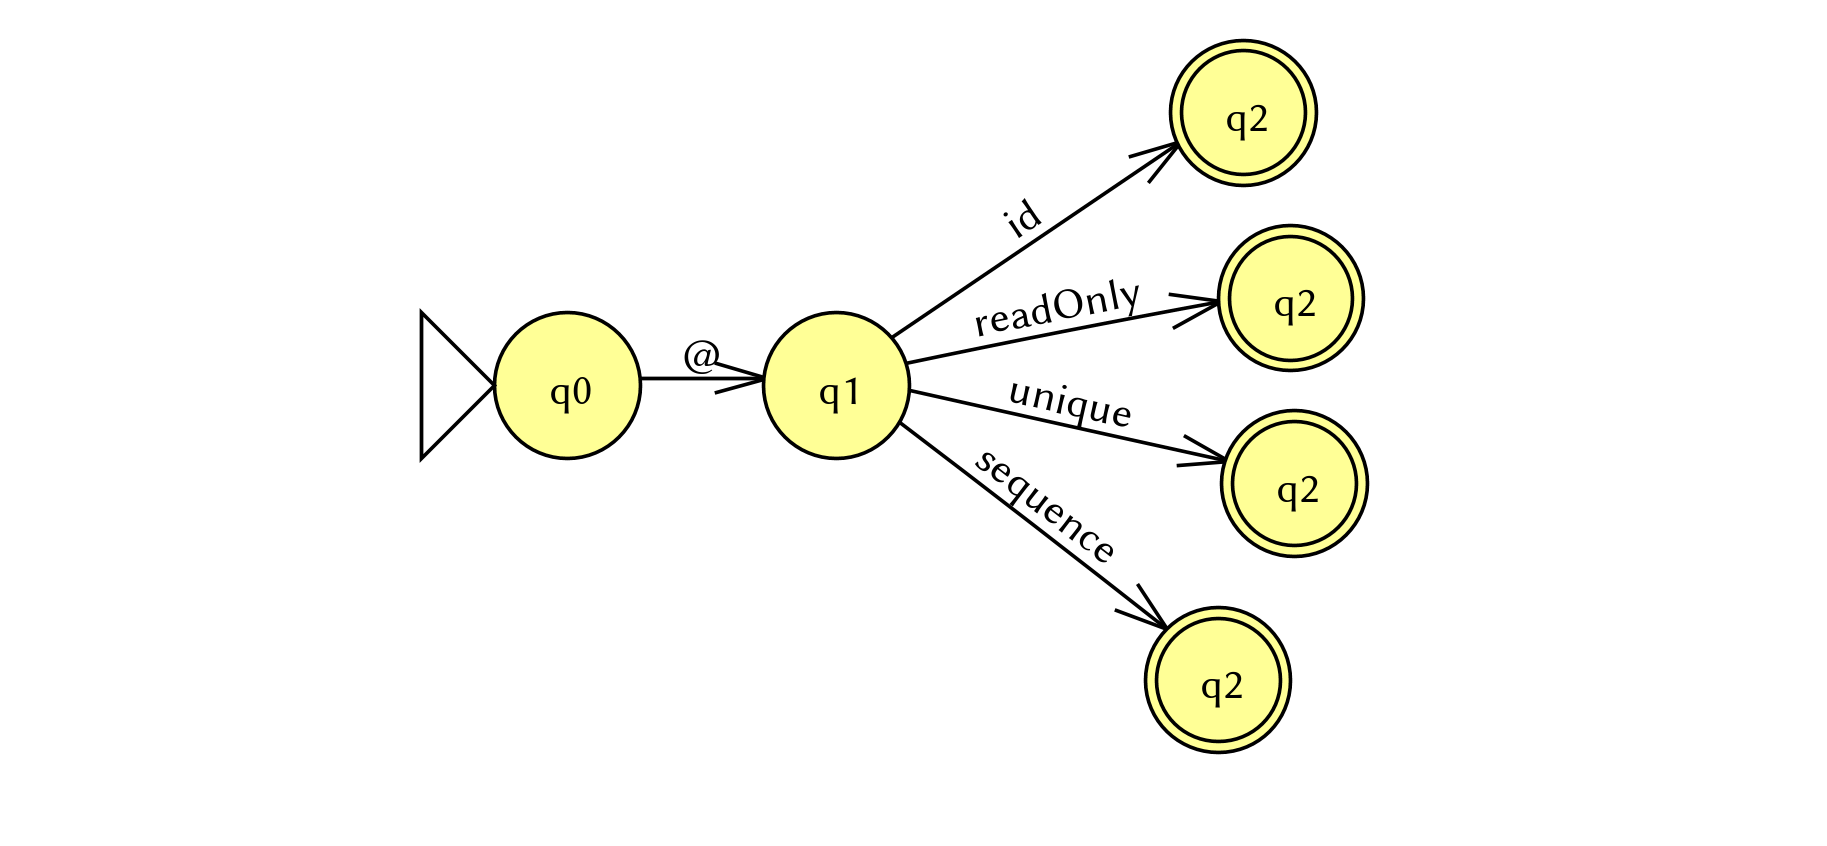
\includegraphics[width=.4\linewidth]{automatas_finitos/modificadores-drt.png}
	\caption{Autómata finito - Modificador para los atributos}
	\label{fig:af_atr_modif_OCL}
\end{figure}
